\documentclass[floatsintext,man]{apa6}

\usepackage{amssymb,amsmath}
\usepackage{ifxetex,ifluatex}
\usepackage{fixltx2e} % provides \textsubscript
\ifnum 0\ifxetex 1\fi\ifluatex 1\fi=0 % if pdftex
  \usepackage[T1]{fontenc}
  \usepackage[utf8]{inputenc}
\else % if luatex or xelatex
  \ifxetex
    \usepackage{mathspec}
    \usepackage{xltxtra,xunicode}
  \else
    \usepackage{fontspec}
  \fi
  \defaultfontfeatures{Mapping=tex-text,Scale=MatchLowercase}
  \newcommand{\euro}{€}
\fi
% use upquote if available, for straight quotes in verbatim environments
\IfFileExists{upquote.sty}{\usepackage{upquote}}{}
% use microtype if available
\IfFileExists{microtype.sty}{\usepackage{microtype}}{}

% Table formatting
\usepackage{longtable, booktabs}
\usepackage{lscape}
% \usepackage[counterclockwise]{rotating}   % Landscape page setup for large tables
\usepackage{multirow}		% Table styling
\usepackage{tabularx}		% Control Column width
\usepackage[flushleft]{threeparttable}	% Allows for three part tables with a specified notes section
\usepackage{threeparttablex}            % Lets threeparttable work with longtable

% Create new environments so endfloat can handle them
% \newenvironment{ltable}
%   {\begin{landscape}\begin{center}\begin{threeparttable}}
%   {\end{threeparttable}\end{center}\end{landscape}}

\newenvironment{lltable}
  {\begin{landscape}\begin{center}\begin{ThreePartTable}}
  {\end{ThreePartTable}\end{center}\end{landscape}}




% The following enables adjusting longtable caption width to table width
% Solution found at http://golatex.de/longtable-mit-caption-so-breit-wie-die-tabelle-t15767.html
\makeatletter
\newcommand\LastLTentrywidth{1em}
\newlength\longtablewidth
\setlength{\longtablewidth}{1in}
\newcommand\getlongtablewidth{%
 \begingroup
  \ifcsname LT@\roman{LT@tables}\endcsname
  \global\longtablewidth=0pt
  \renewcommand\LT@entry[2]{\global\advance\longtablewidth by ##2\relax\gdef\LastLTentrywidth{##2}}%
  \@nameuse{LT@\roman{LT@tables}}%
  \fi
\endgroup}


  \usepackage{graphicx}
  \makeatletter
  \def\maxwidth{\ifdim\Gin@nat@width>\linewidth\linewidth\else\Gin@nat@width\fi}
  \def\maxheight{\ifdim\Gin@nat@height>\textheight\textheight\else\Gin@nat@height\fi}
  \makeatother
  % Scale images if necessary, so that they will not overflow the page
  % margins by default, and it is still possible to overwrite the defaults
  % using explicit options in \includegraphics[width, height, ...]{}
  \setkeys{Gin}{width=\maxwidth,height=\maxheight,keepaspectratio}
\ifxetex
  \usepackage[setpagesize=false, % page size defined by xetex
              unicode=false, % unicode breaks when used with xetex
              xetex]{hyperref}
\else
  \usepackage[unicode=true]{hyperref}
\fi
\hypersetup{breaklinks=true,
            pdfauthor={},
            pdftitle={The effect of linking assumptions and number of response options on inferred scalar implicature rate},
            colorlinks=true,
            citecolor=blue,
            urlcolor=blue,
            linkcolor=black,
            pdfborder={0 0 0}}
\urlstyle{same}  % don't use monospace font for urls

\setlength{\parindent}{0pt}
%\setlength{\parskip}{0pt plus 0pt minus 0pt}

\setlength{\emergencystretch}{3em}  % prevent overfull lines


% Manuscript styling
\captionsetup{font=singlespacing,justification=justified}
\usepackage{csquotes}
\usepackage{upgreek}

 % Line numbering
  \usepackage{lineno}
  \linenumbers


\usepackage{tikz} % Variable definition to generate author note

% fix for \tightlist problem in pandoc 1.14
\providecommand{\tightlist}{%
  \setlength{\itemsep}{0pt}\setlength{\parskip}{0pt}}

% Essential manuscript parts
  \title{The effect of linking assumptions and number of response options on
inferred scalar implicature rate}

  \shorttitle{Linking assumptions and implicature rate}


  \author{Masoud Jasbi\textsuperscript{1}, Brandon Waldon\textsuperscript{1}, \& Judith Degen\textsuperscript{1}}

  % \def\affdep{{"", "", ""}}%
  % \def\affcity{{"", "", ""}}%

  \affiliation{
    \vspace{0.5cm}
          \textsuperscript{1} Stanford University  }

  \authornote{
    Add complete departmental affiliations for each author here. Each new
    line herein must be indented, like this line. Enter author note here.
    
    Correspondence concerning this article should be addressed to Masoud
    Jasbi, Postal address. E-mail:
    \href{mailto:my@email.com}{\nolinkurl{my@email.com}}
  }


  \abstract{Enter abstract here. Each new line herein must be indented, like this
line.}
  \keywords{scalar implicature; methodology; linking assumption; experimental
pragmatics; truth-value judgment task \\

    \indent Word count: X
  }





\usepackage{amsthm}
\newtheorem{theorem}{Theorem}[section]
\newtheorem{lemma}{Lemma}[section]
\theoremstyle{definition}
\newtheorem{definition}{Definition}[section]
\newtheorem{corollary}{Corollary}[section]
\newtheorem{proposition}{Proposition}[section]
\theoremstyle{definition}
\newtheorem{example}{Example}[section]
\theoremstyle{definition}
\newtheorem{exercise}{Exercise}[section]
\theoremstyle{remark}
\newtheorem*{remark}{Remark}
\newtheorem*{solution}{Solution}
\begin{document}

\maketitle

\setcounter{secnumdepth}{0}



\section{Introduction}\label{introduction}

The past 15 years have seen the rise and development of a bustling and
exciting new field at the intersection of linguistics, psychology, and
philosophy: \emph{experimental pragmatics} (Bott \& Noveck, 2004;
Breheny, Katsos, \& Williams, 2006; Degen \& Tanenhaus, 2015; Geurts \&
Pouscoulous, 2009; Grodner, Klein, Carbary, \& Tanenhaus, 2010; Huang \&
Snedeker, 2009; I. A. Noveck \& Reboul, 2008) \textbf{XXX ADD MORE}.
Experimental pragmatics is devoted to experimentally testing theories of
how language is used in context. How do listeners draw inferences about
the -- often underspecified -- linguistic signal they receive from
speakers? How do speakers choose between the many utterance alternatives
they have at their disposal?

The most prominently studied phenomenon in experimental pragmatics is
undoubtedly \emph{scalar implicature}. Scalar implicatures arise in
virtue of a speaker producing the weaker of two ordered scalemates
(hornXXX; {\textbf{???}}, {\textbf{???}}; Grice, 1975). Examples are
provided in (1) and (2).

\begin{enumerate}
\def\labelenumi{\arabic{enumi}.}
\item
\end{enumerate}

\begin{itemize}
\tightlist
\item
  \emph{Utterance:} Some of her pets are cats.
\item
  \emph{Implicature:} Some, but not all, of her pets are cats.
\item
  \emph{Scale:} 
\end{itemize}

\begin{enumerate}
\def\labelenumi{\arabic{enumi}.}
\setcounter{enumi}{1}
\item
\end{enumerate}

\begin{itemize}
\tightlist
\item
  \emph{Utterance:} She owns a cat or a dog.
\item
  \emph{Implicature:} She owns a cat or a dog, but not both.
\item
  \emph{Scale:} 
\end{itemize}

A listener, upon observing the utterances in (1a) and (2a), typically
infers that the speaker intended to convey the meanings in (1b) and
(2b), respectively. Since Grice (1975), the agreed-upon abstract
rationalization the listener could give for their inference goes
something like this: the speaker could have made a more informative
statement by producing the stronger alternative (e.g., \emph{All of her
pets are cats.}). If the stronger alternative is true, they should have
produced it to comply with the Cooperative Principle. They chose not to.
I believe the speaker knows whether the stronger alternative is true.
Hence, it must not be true.

Because the basic reconstruction of the inference is much more easily
characterized for scalar implicatures than for other implicatures,
scalar implicatures have served as a test bed for many questions in
experimental pragmatics, including, but not limited to: 1. Are scalar
inferences default inferences (in the sense of default as arising unless
blocked by marked contexts \textbf{XXX horn, levinson, degen2015)}? 2.
Are scalar inferences default inferences (in the sense that they are
computed automatically in online processing and only cancelled by
context in a second effortful step if required by context)
({\textbf{???}}; Bott \& Noveck, 2004; Breheny et al., 2006; Grodner et
al., 2010; Huang \& Snedeker, 2009)? 3. What are the (linguistic and
extra-linguistic) factors that affect whether a scalar implicature is
derived {[}({\textbf{???}});DegenTanenhaus2015; DegenTanenhaus2016;
Degen2015; DegenGoodman2014; BergenGrodner2012; Breheny2006;
FergusonBreheny2013;DeMarneffeTonhauser;DeNeys2007;Bonnefon{]}? 4. At
what age do children acquire the ability to compute implicatures
{[}Noveck2001; Reboul; Papafragou; Barner; Frank; Musolino{]}?
\textbf{XXX fill in refs}

CONTINUE HERE: motivation for examining implicature rate assumptions:

\begin{itemize}
\item
  surging interest in differences in implicature rates (eg van tiel,
  dgen tanenhaus)
\item
  implicature rates serve as basis for claims about online processing
  (bott \& noveck, degen tanenhaus)
\item
  implicature rates serve as basis for claims about children (bishop
  katsos, barner, frank)
\item
  add ({\textbf{???}})
\item
  ({\textbf{???}}) for investigations of scalar adjectives, and
  ({\textbf{???}})
\end{itemize}

\begin{figure}

{\centering 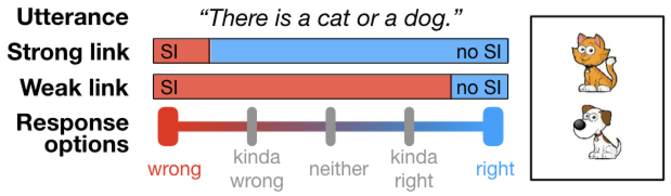
\includegraphics{writeup_files/figure-latex/linkvisualization-1} 

}

\caption{Strong and weak link from response options to researcher inference about scalar implicature rate, exemplified for the disjunctive utterance when the conjunction is true.}\label{fig:linkvisualization}
\end{figure}

\begin{itemize}
\tightlist
\item
  In a truth-value judgment task, how do we know whether an
  interpretation is literal or the result of an implicature computation?
\end{itemize}

Explain the setup * the speaker produces weaker alternative from the
scale * the facts are such that the stronger alternative is true

Traditional Linking Hypotheses: * If an implicature is calculated, the
participant chooses a Non-True/Non-Right response * If an implicature is
calculated, the participant chooses the Wrong/False response * If an
implicature is calculated, the participant chooses the lower end of the
scale (2: wrong/False, 3: wrong, 4: wrong/kinda-wrong, 5:
wrong/kinda-wrong)

Questions: * Do these linking hypotheses give us different measures of
implicature computation? * If they do differ, which one is most stable?

Alternative Linking Hypothesis: * RSA: Response behavior across
conditions (utterance-card combinations) and dependent measures can be
predicted by a linking hypothesis that assumes that participants are
behaving like soft-optimal RSA speakers and provide a particular
response (eg TRUE) to an utterance u if the RSA speaker probability of u
(given the card) is within a particular probability interval (eg, within
the interval {[}theta, 1{]}).

\begin{itemize}
\tightlist
\item
  Differences between traditional approaches and RSA: 1. The traditional
  linking hypotheses are based on a binary implicature/literal theory of
  pragmatic reasoning but RSA gives a continuous measure of pragmatic
  reasoning and allows for better predicting response behavior with
  multiple options.
\end{itemize}

\section{Background}\label{background}

\begin{itemize}
\item
  discussing the ways people in tha past have measured the
  \enquote{implicature rate}.
\item
  it seems like the literature takes the n(not-True)/n(Total) as the
  proporition of responses caused by implicature calculation
\item
  BUT, I remember that Jesse Snedeker said it's NOT n(not-True)/n(Total)
  but it is n(False)/n(Total)
\item
  However, this is probably not a consensus in the field because Katsos
  \& Bishop consider the mid-point response \enquote{big} on the scale
  small-big-huge (strawberry) to be the result of implicture caculation
\item
  what is the most common measure of \enquote{implicature rate} in the
  literature? Binary True/False: Noveck 2001, Chemla \& Spector 2011,
  Ternary: Katsos \& Bishop 2011
\end{itemize}

\section{Methods}\label{methods}

\subsection{Participants}\label{participants}

200 participants were recruited using Amazon Mechanical Turk (binary=50,
ternary53, quaternary=43, quinary=54). No participant was excluded from
the final analysis.

\subsection{Procedure}\label{procedure}

The study was administered online and through Amazon Mechanical Turk.
Participants were introduced to a set of cards with pictures of one or
two animals (Figure \ref{fig:stimuli}). They were told that a
blindfolded fictional character called Bob is going to guess what
animals are on the card. In each trial, participants saw a card as well
as a sentence representing Bob's guess. For example they saw a card with
a cat on it and read the sentence \enquote{there is a cat on the card.}
The study ended after 24 trials. At the end participants were asked
about their\\
You can access and view \href{}{the online study here}.

\subsection{Design and Materials}\label{design-and-materials}

\begin{figure}[t]

{\centering 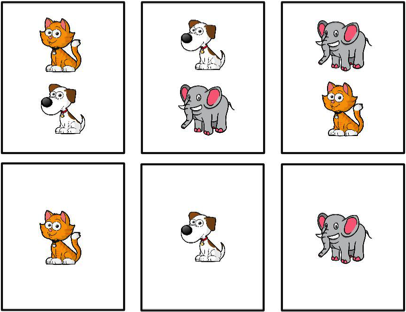
\includegraphics{writeup_files/figure-latex/stimuli-1} 

}

\caption{Cards used in the connective guessing game.}\label{fig:stimuli}
\end{figure}

The design had two main manipulaitons: the type of card and the type of
guess. There were two types of cards. Cards with only one animal on them
and cards with two animals. Animals were chosen from the following set:
cat, dog, and elephant There were three types of guesses: simple (e.g.
\emph{There is a cat}), conjunctive (e.g. \emph{There is a cat and a
dog}), and disjunctive (e.g. \emph{There is a cat or a dog}).

In each trial, the animal labels used in the guess and the animal images
on the card may have no overlap (e.g.~Image: dog, Guess: \emph{There is
a cat or an elephant}), a partial overlap (e.g.~Image: Cat, Guess:
\emph{There is a cat or an elephant}), or a total overlap (e.g.~Image:
cat and elephant, Guess: \emph{There is a cat or an elephant}). Crossing
the number of animals on the card, the type of guess, and the overlap
between the guess and the card results in 12 different possible trial
types. We chose 8 trial types (Figure \ref{fig:trials}), balancing the
number of one-animal vs.~two-animal cards, simple vs.~connective
guesses, and expected true vs.~false trials.

The study used five different types of measurements. 1. two-options
(true vs.~false) 2. two-options (wrong vs.~right) 3. three-options
(wrong, neither, right) 4. four-options (wrong, kinda wrong, kinda
right, right) 5. five-options (wrong, kinda wrong, neither, kinda right,
right).

\begin{figure}[t]

{\centering 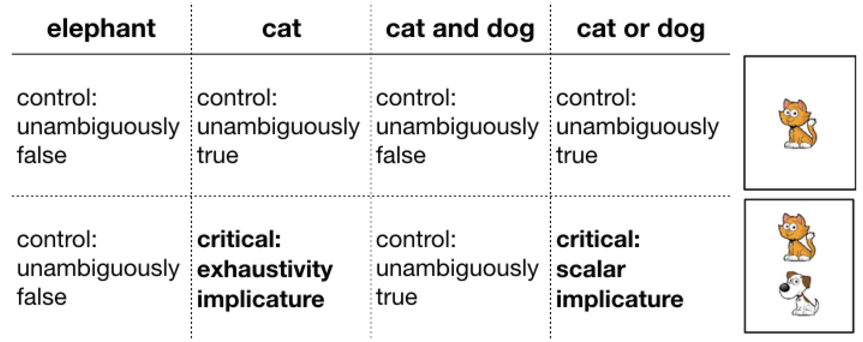
\includegraphics{writeup_files/figure-latex/trials-1} 

}

\caption{Trial types represented by example cards and guesses.}\label{fig:trials}
\end{figure}

\subsection{Pre-registered Analysis}\label{pre-registered-analysis}

We are primarily concerned with the \enquote{rate of implicatures} in an
experimental study. Two trial types are predicted to include pragmatic
implicatures. First, trials where there are two animals on the card but
the fictional character guesses using the connective \emph{or}; for
example \enquote{cat or dog} when the card has both a cat and a dog on
it. We call such trials \enquote{scalar} trials. Second, trials where
there are two animals on the card but the character guesses only one;
for example \enquote{cat} when the card has a cat and a dog on it. We
call such trials \enquote{exhaustive}. In our assessment of implicature
rate we focus on these two types of trials.

We define \enquote{implicature rate} in two ways:

This study set out to test two hypotheses. First, that the proportion of
pragmatic vs.~literal responses in a truth values judgement task changes
based on the number of response options available to the participants.
We test this hypothesis formally using a binomial mixed effects model
with the fixed effect of response type and the random intercept for
participants as well as random intercept and slope for

A second hypothesis was that the definition of what responses count as
participants computing an implicature may affect the estimated rate of
implicature in the experimental task.

\section{Results}\label{results}

\begin{figure}[t]

{\centering 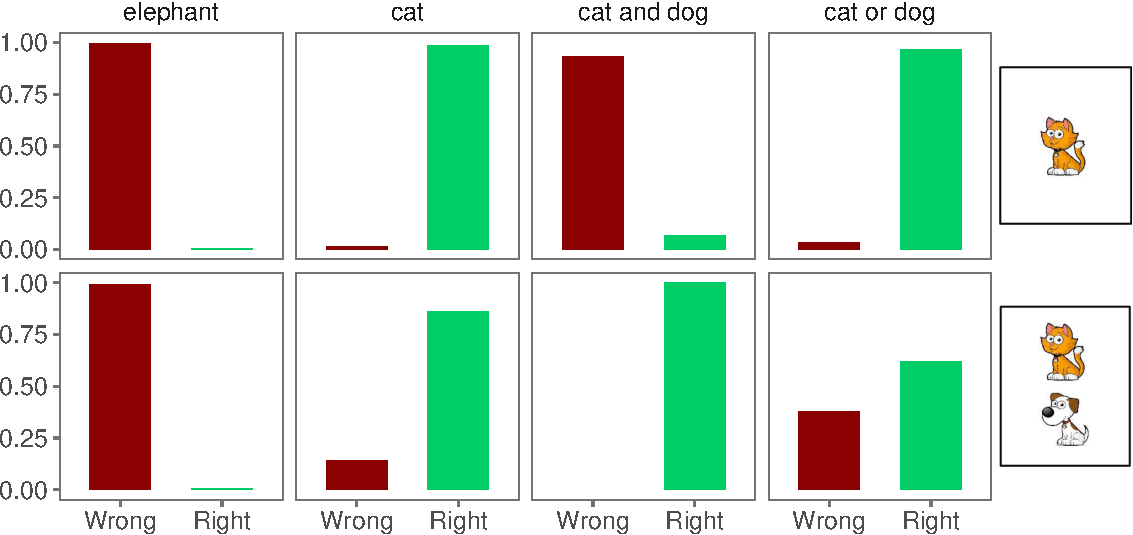
\includegraphics{writeup_files/figure-latex/binaryPlot-1} 

}

\caption{Adults' two-alternative forced choice judgments in the connective guessing game.}\label{fig:binaryPlot}
\end{figure}

\begin{figure}[t]

{\centering 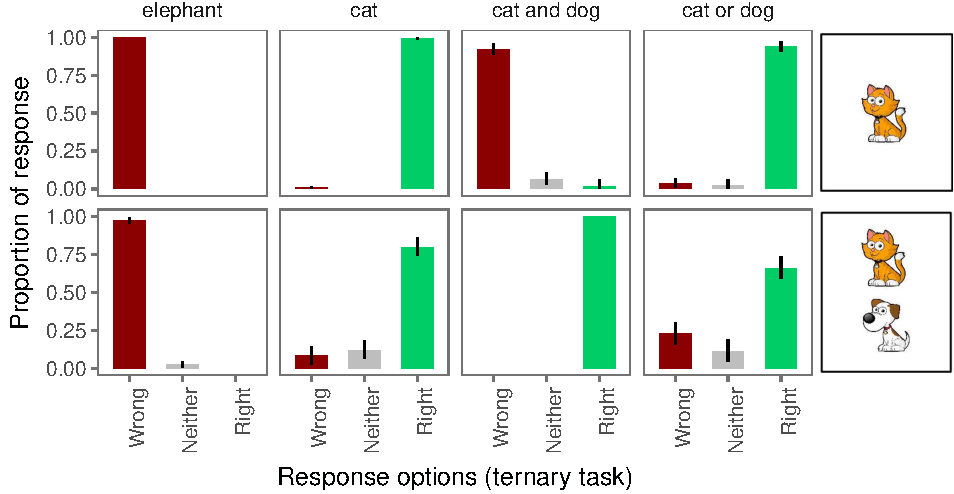
\includegraphics{writeup_files/figure-latex/ternaryPlot-1} 

}

\caption{Adults' three-alternative forced choice judgments in the connective guessing game.}\label{fig:ternaryPlot}
\end{figure}

\begin{figure}[t]

{\centering 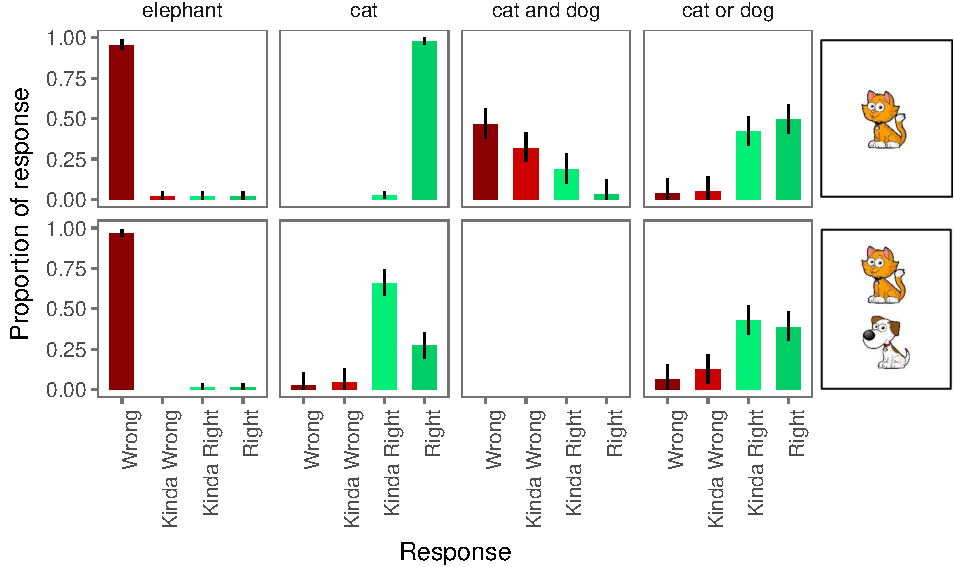
\includegraphics{writeup_files/figure-latex/quaternaryPlot-1} 

}

\caption{Adults' three-alternative forced choice judgments in the connective guessing game.}\label{fig:quaternaryPlot}
\end{figure}

\begin{figure}[t]

{\centering 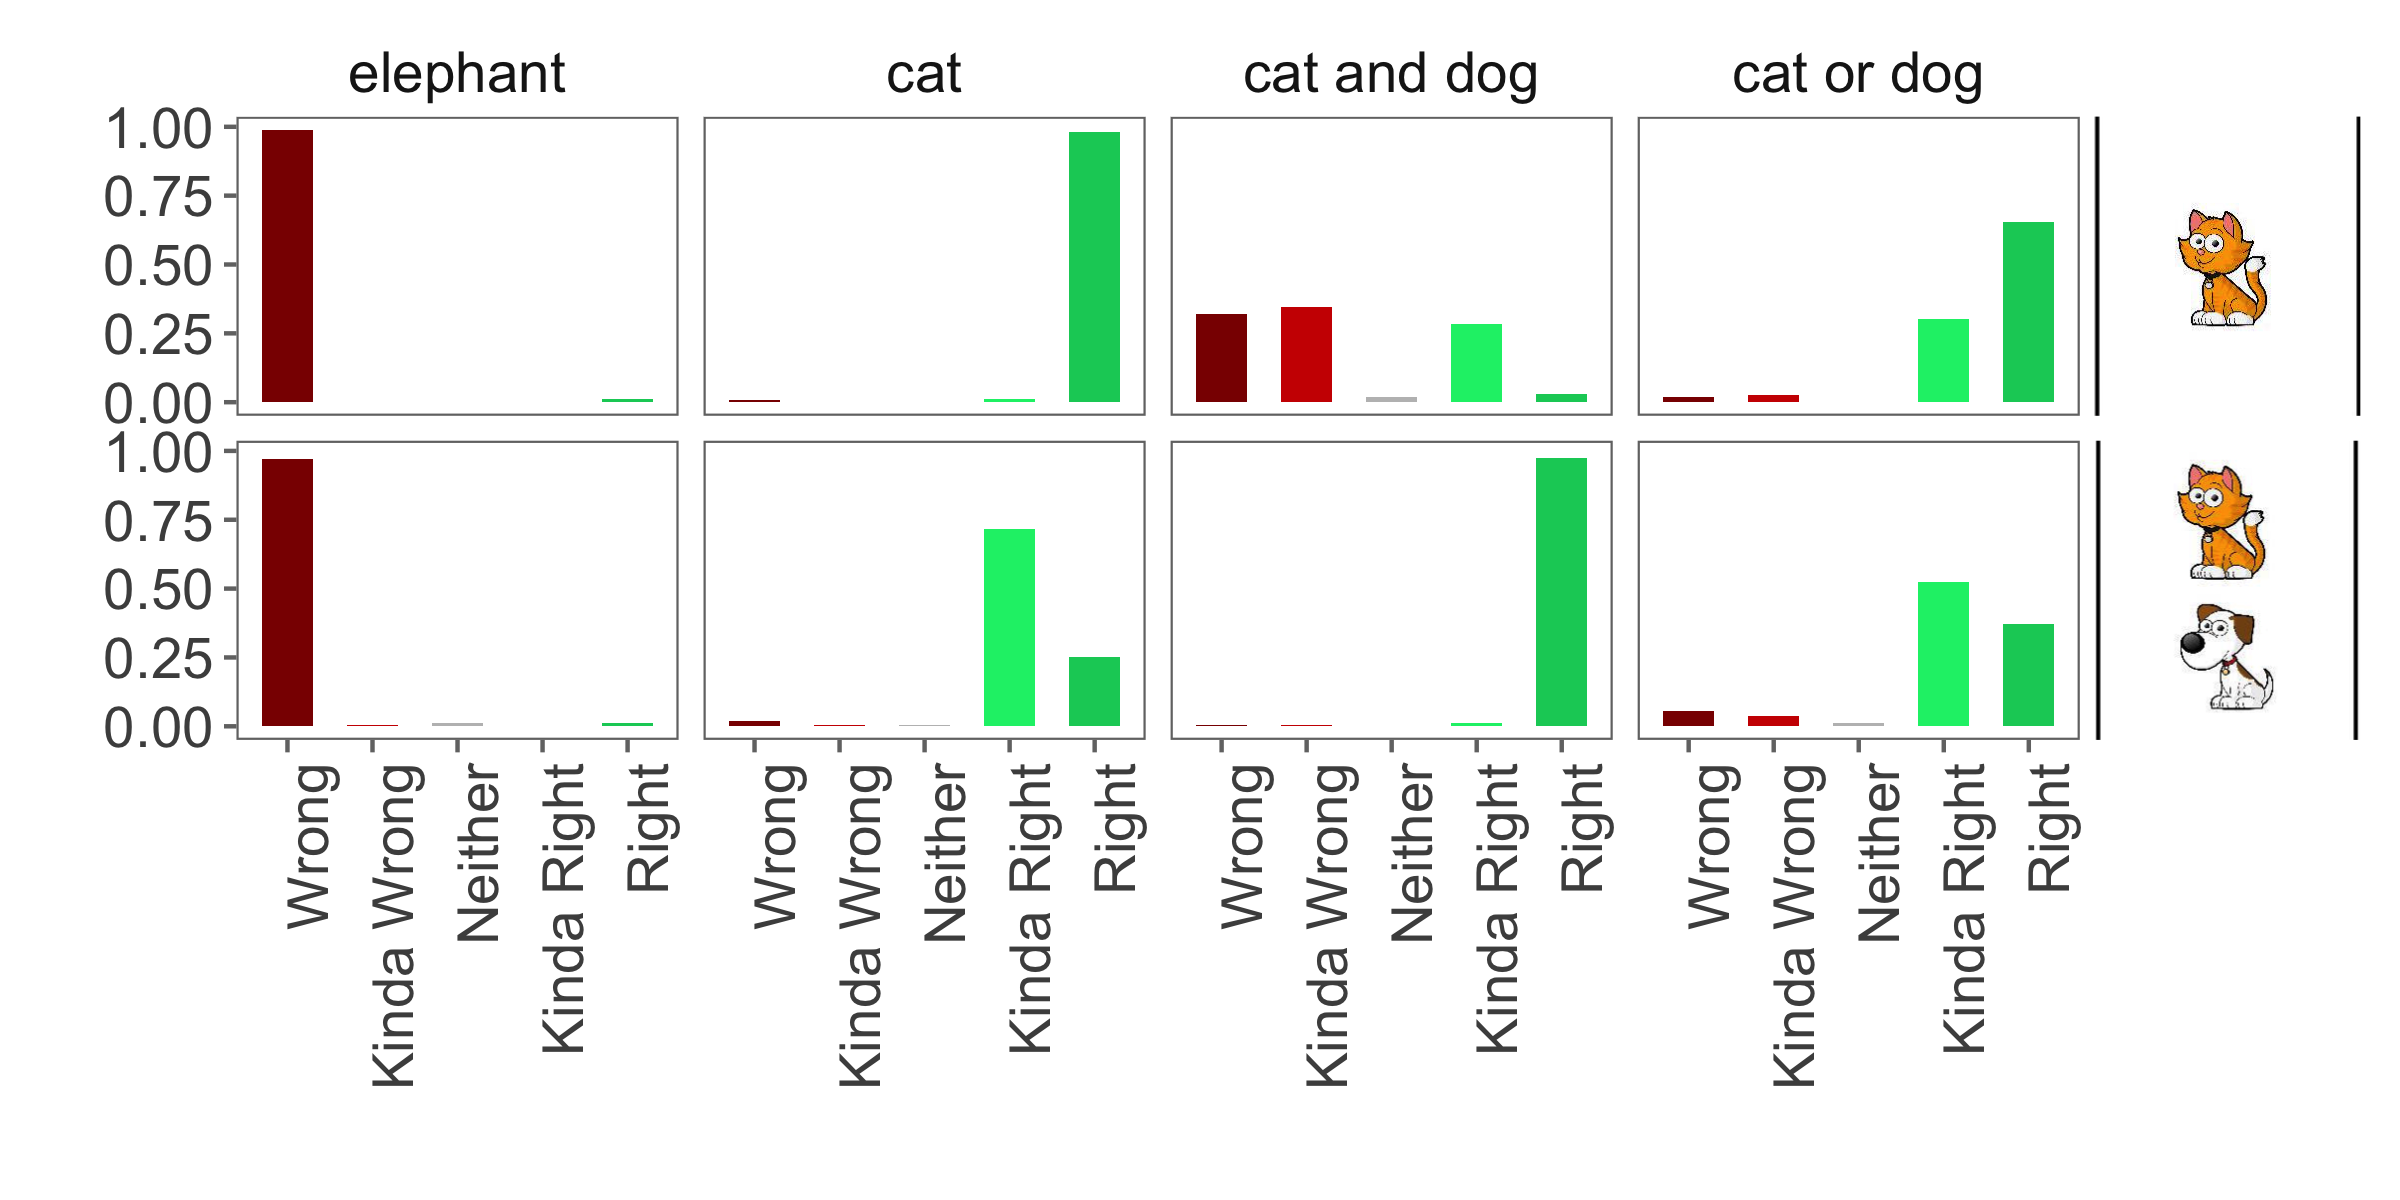
\includegraphics{writeup_files/figure-latex/quinaryPlot-1} 

}

\caption{Adults' three-alternative forced choice judgments in the connective guessing game.}\label{fig:quinaryPlot}
\end{figure}

\begin{figure}
\centering
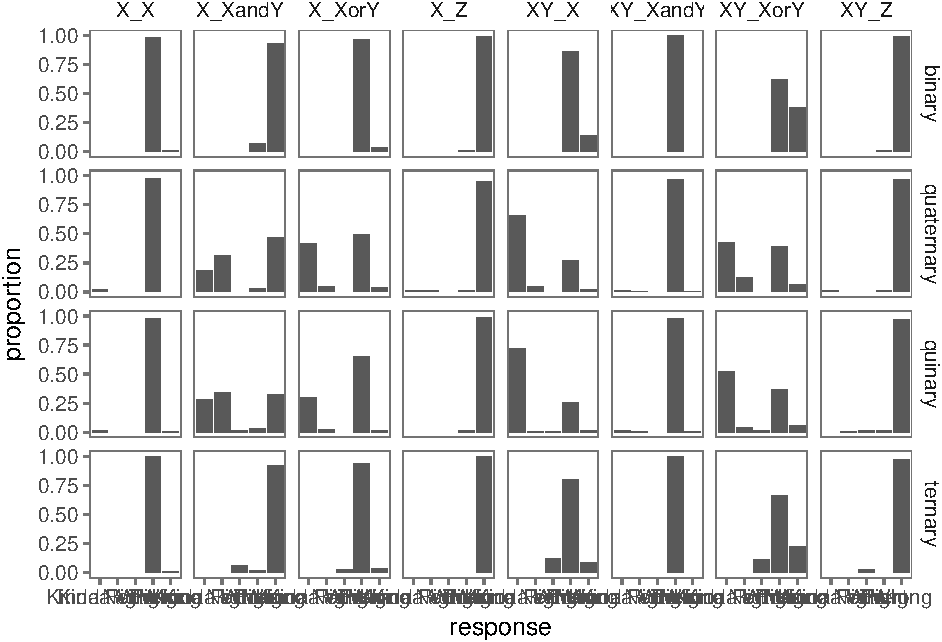
\includegraphics{writeup_files/figure-latex/unnamed-chunk-2-1.pdf}
\caption{}
\end{figure}

\begin{itemize}
\tightlist
\item
  make sure to break down based on whether participants had logical
  training or not.
\end{itemize}

\section{Analysis}\label{analysis}

\begin{figure}
\centering
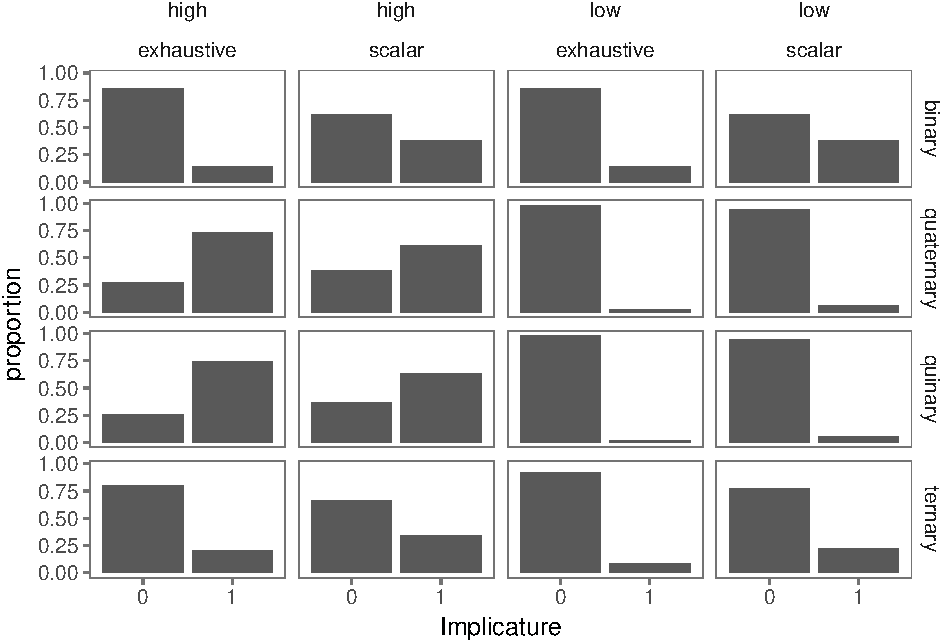
\includegraphics{writeup_files/figure-latex/unnamed-chunk-3-1.pdf}
\caption{}
\end{figure}

\begin{verbatim}
## Warning in (function (fn, par, lower = rep.int(-Inf, n), upper =
## rep.int(Inf, : failure to converge in 10000 evaluations
\end{verbatim}

\begin{verbatim}
## Warning in checkConv(attr(opt, "derivs"), opt$par, ctrl = control
## $checkConv, : Model failed to converge with max|grad| = 0.524298 (tol =
## 0.001, component 1)
\end{verbatim}

\begin{verbatim}
## Generalized linear mixed model fit by maximum likelihood (Laplace
##   Approximation) [glmerMod]
##  Family: binomial  ( logit )
## Formula: implicature ~ definition * response_type + trial_type + (1 +  
##     response_type | card) + (1 | participant)
##    Data: implicature_rate
## 
##      AIC      BIC   logLik deviance df.resid 
##   1783.4   1899.0   -871.7   1743.4     2380 
## 
## Scaled residuals: 
##     Min      1Q  Median      3Q     Max 
## -7.8815 -0.2261 -0.1198  0.2334 10.0887 
## 
## Random effects:
##  Groups      Name                    Variance Std.Dev. Corr             
##  participant (Intercept)             5.224316 2.28568                   
##  card        (Intercept)             0.008402 0.09166                   
##              response_typequaternary 0.084138 0.29007  -1.00            
##              response_typequinary    0.003720 0.06099  -0.79  0.81      
##              response_typeternary    0.044946 0.21201   0.90 -0.89 -0.67
## Number of obs: 2400, groups:  participant, 200; card, 3
## 
## Fixed effects:
##                                       Estimate Std. Error z value Pr(>|z|)
## (Intercept)                           -2.64555    0.43138  -6.133 8.63e-10
## definitionlow                         -0.02508    0.24943  -0.101    0.920
## response_typequaternary                3.47868    0.61328   5.672 1.41e-08
## response_typequinary                   3.44163    0.55426   6.209 5.32e-10
## response_typeternary                   0.29732    0.56967   0.522    0.602
## trial_typescalar                       0.85657    0.13861   6.180 6.41e-10
## definitionlow:response_typequaternary -6.08294    0.61009  -9.970  < 2e-16
## definitionlow:response_typequinary    -5.71913    0.50693 -11.282  < 2e-16
## definitionlow:response_typeternary    -1.21490    0.36931  -3.290    0.001
##                                          
## (Intercept)                           ***
## definitionlow                            
## response_typequaternary               ***
## response_typequinary                  ***
## response_typeternary                     
## trial_typescalar                      ***
## definitionlow:response_typequaternary ***
## definitionlow:response_typequinary    ***
## definitionlow:response_typeternary    ** 
## ---
## Signif. codes:  0 '***' 0.001 '**' 0.01 '*' 0.05 '.' 0.1 ' ' 1
## 
## Correlation of Fixed Effects:
##                     (Intr) dfntnl rspns_typqt rspns_typqn rspns_typt
## definitinlw         -0.287                                          
## rspns_typqt         -0.724  0.202                                   
## rspns_typqn         -0.760  0.224  0.554                            
## rspns_typtr         -0.643  0.218  0.418       0.510                
## trl_typsclr         -0.218 -0.001  0.060       0.065       0.007    
## dfntnlw:rspns_typqt  0.214 -0.408 -0.330      -0.167      -0.101    
## dfntnlw:rspns_typqn  0.217 -0.492 -0.156      -0.309      -0.116    
## dfntnlw:rspns_typt   0.220 -0.675 -0.155      -0.170      -0.280    
##                     trl_ty dfntnlw:rspns_typqt dfntnlw:rspns_typqn
## definitinlw                                                       
## rspns_typqt                                                       
## rspns_typqn                                                       
## rspns_typtr                                                       
## trl_typsclr                                                       
## dfntnlw:rspns_typqt -0.098                                        
## dfntnlw:rspns_typqn -0.103  0.266                                 
## dfntnlw:rspns_typt  -0.036  0.298               0.349             
## convergence code: 0
## Model failed to converge with max|grad| = 0.524298 (tol = 0.001, component 1)
## failure to converge in 10000 evaluations
\end{verbatim}

\section{Modeling}\label{modeling}

\section{Discussion}\label{discussion}

\newpage

\section{References}\label{references}

\setlength{\parindent}{-0.5in} \setlength{\leftskip}{0.5in}

\hypertarget{refs}{}
\hypertarget{ref-bott2004}{}
Bott, L., \& Noveck, I. (2004). Some utterances are underinformative:
The onset and time course of scalar inferences. \emph{Journal of Memory
and Language}, \emph{51}(3), 437--457.
doi:\href{https://doi.org/10.1016/j.jml.2004.05.006}{10.1016/j.jml.2004.05.006}

\hypertarget{ref-Breheny2006}{}
Breheny, R., Katsos, N., \& Williams, J. (2006). Are generalised scalar
implicatures generated by default? An on-line investigation into the
role of context in generating pragmatic inferences. \emph{Cognition},
\emph{100}(3), 434--63.
doi:\href{https://doi.org/10.1016/j.cognition.2005.07.003}{10.1016/j.cognition.2005.07.003}

\hypertarget{ref-DegenTanenhaus2015}{}
Degen, J., \& Tanenhaus, M. K. (2015). Processing scalar implicature A
constraint-based approach. \emph{Cognitive Science}, \emph{39}(4),
667--710.
doi:\href{https://doi.org/10.1111/cogs.12171}{10.1111/cogs.12171}

\hypertarget{ref-Geurts2009}{}
Geurts, B., \& Pouscoulous, N. (2009). Embedded implicatures?!?
\emph{Semantics and Pragmatics}, \emph{2}, 1--34.
doi:\href{https://doi.org/10.3765/sp.2.4}{10.3765/sp.2.4}

\hypertarget{ref-grice1975}{}
Grice, H. P. (1975). Logic and Conversation. \emph{Syntax and
Semantics}, \emph{3}, 41--58. Retrieved from
\href{http://books.google.com/books?hl=en\%7B/\&\%7Dlr=\%7B/\&\%7Did=hQCzOmaGeVYC\%7B/\&\%7Doi=fnd\%7B/\&\%7Dpg=PA121\%7B/\&\%7Ddq=Logic+and+conversation\%7B/\&\%7Dots=j7aijUymwm\%7B/\&\%7Dsig=iV1rz1eEm4ns6bQ6CevIURXFVO4}{http://books.google.com/books?hl=en\{\textbackslash{}\&\}lr=\{\textbackslash{}\&\}id=hQCzOmaGeVYC\{\textbackslash{}\&\}oi=fnd\{\textbackslash{}\&\}pg=PA121\{\textbackslash{}\&\}dq=Logic+and+conversation\{\textbackslash{}\&\}ots=j7aijUymwm\{\textbackslash{}\&\}sig=iV1rz1eEm4ns6bQ6CevIURXFVO4}

\hypertarget{ref-Grodner2010}{}
Grodner, D. J., Klein, N. M., Carbary, K. M., \& Tanenhaus, M. K.
(2010). ``Some,'' and possibly all, scalar inferences are not delayed:
Evidence for immediate pragmatic enrichment. \emph{Cognition},
\emph{116}(1), 42--55.
doi:\href{https://doi.org/10.1016/j.cognition.2010.03.014}{10.1016/j.cognition.2010.03.014}

\hypertarget{ref-huang2009}{}
Huang, Y. T., \& Snedeker, J. (2009). On-line interpretationf of scalar
quantifiers: Insight into the semantics-pragmatics interface.
\emph{Cognitive Psychology}, \emph{58}, 376--415.

\hypertarget{ref-noveck2008}{}
Noveck, I. A., \& Reboul, A. (2008). Experimental pragmatics: a Gricean
turn in the study of language. \emph{Trends in Cognitive Sciences},
\emph{12}(11), 425--431.
doi:\href{https://doi.org/10.1016/j.tics.2008.07.009}{10.1016/j.tics.2008.07.009}






\end{document}
